\documentclass[12pt, a4paper]{article}

\usepackage{amsmath}
\usepackage[utf8]{inputenc}
\usepackage[brazil]{babel}
\usepackage{microtype}
\usepackage{indentfirst}
\usepackage{graphicx}
\usepackage{booktabs}
\usepackage[style=abnt, backend=biber]{biblatex}
\usepackage{csquotes}
\addbibresource{Referencias.bib}
\usepackage{times}

\title{Relatório ITP}
\author{Thiago Oliveira Coelho}

\begin{document}

\maketitle

\tableofcontents

\clearpage

\section{Introdução}

\subsection{As barreiras não tarifárias ao comércio}
Com o advento da globalização o valor das tarifas internacionais tem caído ao longo do tempo, isto diminui as oportunidades para implementação de medidas protecionistas \cite{maskus2000quantifying}. O foco passa então a ser as barreiras não tarifárias (BNTs), conjunto de fatores não tarifários que impedem o fluxo de bens internacionais. Dentre as barreiras não tarifárias são inclusas as normas as quais os produtores devem se conformar para exportar para determinado país. Tais normas devem ser comunicadas aos demais países por meio de notificações, e são regulamentadas pela Organização Mundial do Comércio (OMC). Elas podem ser sanitárias ou fitossanitárias (SPS), associadas a produtos alimentícios, ou barreiras técnicas ao comércio (TBT), que ditam regras para que o produto se adeque ao mercado interno.

Apesar de tais barreiras poderem ser legítimas, por exemplo para corrigir eventuais externalidades negativas advindas do produto importado,  o fato é que estas terão impacto no comércio do país. Este impacto pode ser positivo ou negativo, dependendo do setor afetado, do objetivo da notificação e de seu conteúdo. Os acordos SPS e TBT possuem o objetivo de:

\begin{itemize}
    \item Encorajar membros a adequar seus produtos com base em regulamentações internacionais, visando melhor facilidade ao comércio internacional;
    \item Impedir a criação de barreiras arbitrárias e que não possuam embasamento científico;
    \item Manter a soberania do país para especificar normas de acordo com sua situação específica, desde que estas não visem prejudicar o fluxo de bens internacional;
    \item Exigir que novas normas que afetem o comércio sejam notificadas aos demais países, e que "pontos focais" devem ser estabelecidos. Estes são escritórios que visam melhorar a  transparência das normas estabelecidas pelo país em questão. O ponto focal brasileiro é o Inmetro.
\end{itemize}

Em geral a literatura  nos diz que normas de importação tendem a diminuir o comércio para bens primários e impulsionar o comércio de bens mais complexos \cite{moenius}. Regulamentações particularmente informativas irão diminuir a incerteza em tais transações, porém acompanhar tais notificações pode ser difícil para o micro e pequeno participante do agronegócio. 

O presente trabalho visa explorar os impactos das notificações relacionadas a normas sanitárias e fitossanitárias  (SPS) e barreiras técnicas  (TBT) na exportação de produtos agropecuários. Por isso utilizaremos o valor de exportação somente dos produtos presentes nos 15 primeiros capítulos do sistema harmonizado de categorização. As notificações são categorizadas de acordo com seu objetivo, e é a partir de tal objetivo que distinguiremos os diferentes tipos de notificações e seus respectivos impactos.

\subsection{A relação das barreiras técnicas com o setor agroexportador} \label{barreiras}

Levando em conta a estrutura de exportações do brasil:

\begin{figure}[h]
    \centering
    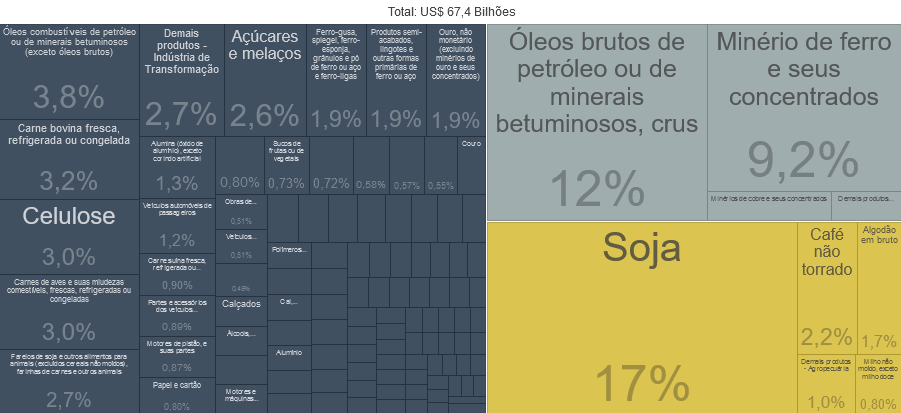
\includegraphics[scale=0.65]{Imagens/ComexStat.PNG}
    \caption{Exportações Brasileiras por produto de Janeiro a junho de 2020. \newline Fonte: \cite{ComexStat}}
\end{figure}

Vemos que grande parte das exportações brasileiras estão relacionadas ao setor agropecuário: soja com 19\%, carne bovina com 3,2\%, café com 2,2\% e algodão com 1,7\%. Pela importância de tais categorias, é importante identificarmos eventuais gargalos a sua comercialização, entre estes as barreiras não tarifárias. Para observarmos  tais impactos iremos separar as notificações emitidas em categorias diferentes dependendo de seus objetivos e analisar o impacto de suas emissões sobre o valor de exportação do Brasil no mesmo período. Nossos resultados serão dispostos de modo a exibir o que influencia a exportação dos 15 primeiros capítulos do sistema harmonizado em agregado, e depois analisaremos alguns dos capítulos mais importantes de acordo com a caracterização das exportações brasileiras.

\newpage

\subsection{Papel governamental na diminuição de gargalos}

\begin{figure}[h]
    \centering
    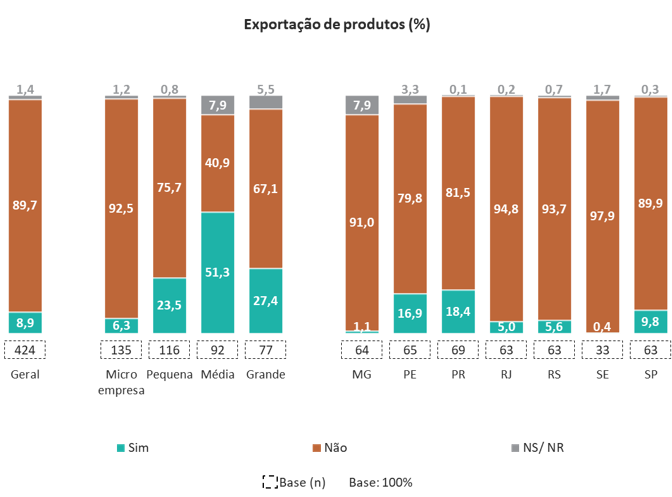
\includegraphics[scale=0.75]{Imagens/Exportacao_2.PNG}
    \caption{Caracterização de empresas exportadoras 
    Fonte: Pesquisa de Demanda INNOVARE}
\end{figure}

Em geral é possível perceber que as micro empresas e de pequeno porte não exportam. Como este trabalho irá desenvolver, existem gargalos relacionados a normas técnicas que podem criar desincentivos a comercialização de bens nacionais para o exterior, e tais gargalos podem afetar empresas menores desproporcionalmente. Por isso é de grande importância a existência de instituições como as da rede sibratec, que por meio da inovação tecnológica e prestação de serviços visam equalizar a competição, oferecendo melhores oportunidades para o micro e pequeno empresário.

\section{Metodologia}

Serão utilizados modelos econométricos de gravidade, que por meio de cálculos Poisson Pseudo Maximum Likelihood (PPML), irão retornar coeficientes para cada variável do modelo. Assim podemos observar os efeitos que cada variável possui sobre os fluxos exportadores brasileiros.

\subsection{Modelos de gravidade}

Os modelos de gravidade são utilizados majoritariamente desde a década de 60 para a explicação de fluxos de comércio internacional. Originalmente derivado do modelo de Newton, utilizava a distância entre os dois objetos (países) e a massa deles (PIB), para explicar tal fluxo. Com o tempo, o desenvolvimento da área de economia internacional têm tornado o modelo cada vez mais teóricamente embasado e representativo da realidade, incluindo diversas variáveis como população, tarifas e efeitos fixos para unidade temporal e país \cite{nascimento2013evoluccao}.

\subsection{Estimador PPML}
Considerando os trabalhos que visam estabelecer quantitativamente o impacto das notificações (\cite{impactosprodquimicos} e \cite{ALMEIDA2014}), será utilizado um modelo de gravidade cujos estimadores serão estabelecidos por PPML (Poisson Pseudo Maximum Likelihood). Tal modo de estimação permite menor viés ao trabalharmos com fluxos internacionais, visto que muitas das observações de emissão de notificações ou de tarifas podem ser de valor nulo. Um modelo de regressão estimado por mínimos quadrados ordinários não está preparado para lidar com tais fluxos zero, o que deixa o resultado enviesado \cite{Log_Of_Gravity}.

\subsection{Software}
Foi utilizado o pacote GME, escrito na linguagem de programação Python pela USITC (United States Internacional Trade Commission). Tal pacote roda diagnósticos da ppml para confirmar que não houve erros na estimação, além de permitir a fácil inclusão dos efeitos fixos e da estimação setor por setor.

\subsection{Variáveis do modelo}

\begin{equation}
    \ln X_{D} = 
    \ln GDP_{O} 
    + \ln GDP_{D} 
    + \ln dist 
    + \ln Tariff 
    + \sum_{i=1}^{n} P 
    % + Eu_{D} 
    + contig 
    % + comrelig
    % + gatt_o 
    % + gatt_D
\end{equation}

Onde:

\begin{itemize}
    \item $X$ = Valor de exportação do Brasil para o país de destino no período;
    \item $GDP_{O}$ = Produto interno bruto nominal do Brasil no período;
    \item $GDP_{D}$ = Produto interno bruto nominal do país de destino no período;
    \item $dist$ = Distância em Quilômetros  do Brasil para o país de destino;
    \item $Tariff$ = Média ponderada das tarifas efetivamente aplicadas pelo país de destino ao Brasil no período;
    \item $\sum_{i=1}^{n} P$ = Conjunto de variáveis que indicam a quantidade de notificações emitidas por cada país e objetivo;
    % \item $Eu_{D}$ = Dummy que indica se o país de destino faz parte da União Europeia.
    \item $contig$ = Dummy que indica se o Brasil possui fronteiras em comum com o país de destino;
    % \item $comrelig$ = Dummy que indica se os países possuem religiões difundidas em comum;
    % \item $gatt_O$ = Se o país (origem) é membro da Organização mundial do comércio;
    % \item $gatt_D$ = Se o país (destino) é membro da Organização mundial do comércio.
\end{itemize}

Esta equação resume que as alterações percentuais no valor de exportações brasileiras são dependentes do PIB do Brasil e do país importador, da distância e existência de fronteiras em comum entre os dois, e da emissão ou não de diversos tipos de notificações naquele substrato de tempo. O período utilizado na análise é anual.

\subsection{Dados e fontes}

Bases de dados utilizadas:

\begin{enumerate}
    \item Notificações: Sistema de alerta de notificações EPING: https://www.epingalert.org/en;
    \item Valor de exportações: Base de dados estatísticos sobre comércio internacional das Nações Unidas: https://comtrade.un.org/;
    \item PIB: Sistema de dados abertos do banco mundial: https://data.worldbank.org/;
    \item Distância e fronteiras em comum: Base de dados para modelos gravitacionais da Centre d'Etudes Prospectives et d'Informations Internationales: \cite{CEPII};
    \item Tarifas: WITS (World Integrated Trade Solution): https://wits.worldbank.org/.
\end{enumerate}

\subsection{Interpretação}

Pela natureza do estimador não tão utilizado e do fato de estarmos lidando com um modelo em logaritmo, algumas precauções quanto a interpretação do modelo são necessárias:

\subsubsection{Coeficientes}

Os coeficientes representam impactos percentuais nas exportações dada alteração de 1 ponto percentual na variável explicativa, por exemplo de 5\% para 6\%. Isso se dá pelo fato das variáveis estarem logaritmadas, mas não no caso das variáveis relacionadas a notificações. Como o logaritmo natural de 0 é indefinido e muitos objetivos de notificações possuem valor 0 para certos anos, logaritmar tal variável prejudicaria a acurácia do modelo. O valor exato da alteração causado pelas notificações portanto é de difícil interpretação, e é recomendável que o valor de tais coeficientes seja utilizado para determinar somente se o impacto de tal tipo de notificação é positivo ou negativo.

\subsubsection{P-Valor}
O p-valor é uma medida estatística simples que nos indica a relevância de uma variável aos diversos níveis de significância. Nos dá uma probabilidade de encontrarmos uma amostra mais representativa da realidade do que a que temos atualmente. Se o p-valor de uma variável for menor que o valor decimal do nível de significância escolhido, podemos concluir que tal variável rejeita a hipótese nula, que nos diz que a variável independente não impacta a variável dependente (exportações). Sendo assim:

\begin{itemize}
    \item $P < 0.1$ : variável significativa a $10\%$;
    \item $P < 0.05$ : variável significativa a $5\%$;
    \item $P < 0.01$ : variável significativa a $1\%$.
    \item $P < 0.001$ : variável significativa a $0.1\%$.
\end{itemize}

Quanto menor o p-valor, maior a confiança de que uma variável é significativa. Em geral o nível de significância utilizado por padrão é $5\% (p-valor < 0.05)$.


\newpage
\section{Resultados}

\subsection{Regressão com efeitos fixos e setores agregados}

\begin{table}[ht]
\begin{center}
        
        \begin{tabular}{lcccccc}
            & \textbf{coef} &\textbf{P$> |$t$|$}\\
\midrule
\textbf{Animal.health}                                             &      -0.0044 &        0.097       \\
\textbf{Consumer.information}                                      &       0.0818 &        0.049       \\
\textbf{Food.safety}                                               &       0.0028 &        0.356       \\
\textbf{Harmonization}                                             &       1.6080 &        0.000       \\
\textbf{Lower.barriers.to.trade}                                   &       0.0264 &        0.743       \\
\textbf{Other}                                                     &      43.9902 &        0.000       \\
\textbf{Plant.protection}                                          &      -0.0111 &        0.007       \\
\textbf{Prevention.of.deceptive.practices.and.consumer.protection} &       0.0104 &        0.365       \\
\textbf{Protect.humans.from.animal.plant.pest.or.disease}          &      -0.0016 &        0.678       \\
\textbf{Protect.territory.from.other.damage.from.pests}            &      -0.0115 &        0.248       \\
\textbf{Protection.of.Human.health.or.Safety}                      &      -0.0089 &        0.034       \\
\textbf{Protection.of.animal.or.plant.life.or.health}              &      -0.1620 &        0.000       \\
\textbf{Protection.of.the.environment}                             &      -0.4332 &        0.000       \\
\textbf{Quality.requirements}                                      &      -0.0109 &        0.508       \\
\textbf{ln\_gdp\_d}                                                &       0.0837 &        0.202       \\
\textbf{ln\_gdp\_o}                                                &      94.2923 &        0.000       \\
\textbf{comrelig}                                                  &      43.6092 &        0.008       \\
\textbf{gatt\_d}                                                   &      -1.0816 &        0.003       \\
\textbf{gatt\_o}                                                   &   -2764.3993 &        0.000       \\
\textbf{eu\_d}                                                     &      -3.3776 &        0.012       \\
\textbf{ln\_dist}                                                  &       7.9788 &        0.018       \\
\textbf{contig}                                                    &       0.0207 &        0.456       \\
\textbf{ln\_Tariff}                                                &       0.0147 &        0.031       \\
\bottomrule
\end{tabular}
\end{center}
\caption{Resultado Modelo CEPII}
\end{table}

 Utilizando 5\% como corte para a significância, vamos isolar as variáveis significativas relacionadas as notificações :

 \begin{itemize}
         \item Harmonização: Impacto positivo;
         \item Proteção de plantas: Impacto negativo;
         \item Proteger território de dano por pestes: Impacto negativo;
         \item Proteção do meio ambiente: Impacto negativo.
         \item Proteção da saúde animal ou vegetal: Impacto negativo;
         \item Informação ao consumidor: Impacto positivo;
 \end{itemize}

 As variáveis de informação ao consumidor e harmonização possuem impacto positivo sobre as exportações brasileiras. Isso condiz com a literatura, que afirma que as notificações informativas ao exportador beneficiam o comércio por caracterizar aspectos importantes do mercado externo. A variável harmonização, por exemplo, visa a adequação das regras de comércio em bases internacionais, equalizando as normas e deixando o ambiente mais competitivo.

Podemos perceber que as variáveis relacionadas a proteção são as que impactam negativamente o comércio internacional. Isso pode significar que a adaptação dos produtos a esta pode ser particularmente difícil ou cara, o que seria compreensível, visto que tenderiam a ser mais rigorosas. A variável proteção ao meio ambiente, significativa a nível de 0.1\% pode significar possível oportunidade para execução de serviços relacionadas ao laboratórios da rede. Tais variáveis podem nos ajudar a explicar o fato de que empresas de menor porte tendem a nao ser exportadoras. É mais compreensível que suas estruturas de custo não suportem aumentos muito significativos que venham a ser necessários para exportar seus produtos.

Considerando as variáveis não relacionadas com notificações: as de PIB foram ambas significativas e positivas, ou seja, aumentos na renda tanto do Brasil quanto do importador acarretam em maiores exportações. As variáveis que buscavam serem \emph{proxys} dos custos explícitos de exportação, como a distância, as fronteiras em comum e o valor efetivamente aplicado das tarifas tiveram resultados interessantes. A distância entre países foi significativa, e apresentou coeficiente negativo, o que condiz com a literatura: quanto maior a distância menor tende a ser o comércio entre os países. A variável \emph{contig}, que expressa se o país importador faz fronteira com o Brasil no entanto foi não significativa a 5\% e teve coeficiente negativo, o que não seria um comportamento esperado, especialmente levando em conta a variável anterior que nos diz que a distância tem relação negativa com o comércio. Porém analisando trabalhos parecidos, como \cite{ALMEIDA2014}, que faz medição semelhante porém desagregada para cada produto, observamos que isso pode ocorrer. No trabalho, os seguintes itens apresentam comportamento parecido:

\begin{itemize}
    \item Carne Bovina e miudezas de carnas curadas: Não significante;
    \item Cortes bovinos, desossados e congelados: Significante e com impacto negativo;
    \item Frango em pedaços congelado: Não significativo;
    \item Óleo de soja Bruto: Não significativo;
    \item Café verde, não torrado e não descafeinado: Significativo e com impacto negativo.
\end{itemize}

Percebe-se que todos estes produtos estão inclusos em nossa análise, que leva em conta os primeiros 15 capítulos do sistema harmonizado, todos estes ligados a produtos agropecuários. Tal comportamento portanto não seria em todo anormal. A variável de tarifas efetivamente aplicadas foi significativa somente a 10\% e teve coeficiente positivo, novamente contrariando o que seria deduzindo comumente. Segundo o mesmo trabalho citado acima, as tarifas tiveram impactos positivos para o comércio de soja, que, como exposto na seção \ref{barreiras} representa maior parte da exportação brasileira. Portanto, ao agregarmos estes vários produtos a maior representabilidade da soja pode ter enviesado os resultados.

\subsection{Regressão sem efeitos fixos e resultados setor por setor}


\subsubsection{Setor 01 - Animais vivos}


\begin{center}
\begin{tabular}{lcccccc}
                                                          & \textbf{Coeficiente} & \textbf{Erro padrão} &\textbf{P$> |$t$|$}\\
\midrule
\textbf{Animal.health}                                    &       0.0233  &        0.045     &        0.604     \\
\textbf{Food.safety}                                      &       0.0177  &        0.053     &        0.737     \\
\textbf{Plant.protection}                                 &       0.0472  &        0.061     &        0.440     \\
\textbf{Protect.humans.from.animal.plant.pest.or.disease} &       0.0478  &        0.060     &        0.425     \\
\textbf{Protect.territory.from.other.damage.from.pests}   &       0.0816  &        0.107     &        0.447     \\
\textbf{ln\_gdp\_d}                                       &       0.0247  &        0.028     &        0.379     \\
\textbf{ln\_gdp\_o}                                       &     226.9168  &       73.469     &        0.002     \\
\textbf{comrelig}                                         &       0.1864  &        0.205     &        0.363     \\
\textbf{gatt\_d}                                          &   -6451.3982  &     2089.756     &        0.002.043 \\
\textbf{ln\_dist}                                         &      -0.0316  &        0.086     &        0.713     \\
\textbf{contig}                                           &      -0.1325  &        0.156     &        0.395     \\
\textbf{ln\_Tariff}                                       &      -0.0145  &        0.041     &        0.722     \\
\bottomrule
\end{tabular}
%\caption{Generalized Linear Model Regression Results}
\end{center} 

Variáveis  significativas a 5\%:
\begin{itemize}
    \item Food.safety: $0.0606$;
    \item Protect.humans.from.animal.plant.pest.or.disease: $-0.1003$;
    \item Protect.territory.from.other.damage.from.pests: $0.1847$;
\end{itemize}

Surpreendentemente as notificações que objetivam saúde animal não foram significativas. Temos que as notificações para segurança relacionada a comida e proteção de território a dano de pestes possuem impacto negativo. A proteção de seres humanos a doenças relacionadas a plantas ou animais foi a única variável relacionada a notificações que impacta negativamente o comércio deste setor. 

\subsubsection{Setor 02 - Carnes e miudezas, comestíveis}


\begin{center}
\begin{tabular}{lcccccc}
                                                          & \textbf{coef} & \textbf{std err} & \textbf{t} & \textbf{P$> |$t$|$} & \textbf{[0.025} & \textbf{0.975]}  \\
\midrule
\textbf{Animal.health}                                    &      -0.0249  &        0.025     &    -0.993  &         0.321        &       -0.075    &        0.025     \\
\textbf{Food.safety}                                      &       0.0015  &        0.009     &     0.165  &         0.869        &       -0.017    &        0.020     \\
\textbf{Plant.protection}                                 &      -0.0515  &        0.051     &    -1.008  &         0.313        &       -0.153    &        0.050     \\
\textbf{Protect.humans.from.animal.plant.pest.or.disease} &       0.0032  &        0.022     &     0.142  &         0.887        &       -0.041    &        0.047     \\
\textbf{Protect.territory.from.other.damage.from.pests}   &       0.0097  &        0.036     &     0.269  &         0.788        &       -0.062    &        0.081     \\
\textbf{Protection.of.Human.health.or.Safety}             &      -0.0689  &        0.015     &    -4.537  &         0.000        &       -0.099    &       -0.039     \\
\textbf{ln\_gdp\_d}                                       &       0.0167  &        0.007     &     2.422  &         0.015        &        0.003    &        0.030     \\
\textbf{ln\_gdp\_o}                                       &       0.1083  &        0.077     &     1.405  &         0.160        &       -0.045    &        0.261     \\
\textbf{comrelig}                                         &      -0.3257  &        0.088     &    -3.684  &         0.000        &       -0.501    &       -0.150     \\
\textbf{gatt\_d}                                          &      -0.0354  &        0.083     &    -0.428  &         0.668        &       -0.199    &        0.128     \\
\textbf{gatt\_o}                                          &      -0.2182  &        2.176     &    -0.100  &         0.920        &       -4.531    &        4.094     \\
\textbf{eu\_d}                                            &       0.1440  &        0.043     &     3.366  &         0.001        &        0.059    &        0.229     \\
\textbf{ln\_dist}                                         &      -0.0454  &        0.063     &    -0.725  &         0.468        &       -0.169    &        0.079     \\
\textbf{contig}                                           &       0.0834  &        0.091     &     0.917  &         0.359        &       -0.097    &        0.264     \\
\textbf{ln\_Tariff}                                       &       0.0366  &        0.015     &     2.407  &         0.016        &        0.006    &        0.067     \\
\bottomrule
\end{tabular}
%\caption{Generalized Linear Model Regression Results}
\end{center} 

A única variável relacionada as notificações significativa a 5\% foi a de proteção a saúde e segurança humana, com coeficiente de $-0.0689$. Novamente conferimos que tais variáveis de proteção a saúde e ao meio ambiente são as que mais impactam negativamente o comércio destas commodities.

\newpage

\subsubsection{Setor 03 - Peixes e crustáceos, moluscos e outros invertebrados aquáticos}



\begin{table}[ht!]
    \begin{center}
        \begin{tabular}{lcccccc}
            & \textbf{Coeficiente} &\textbf{P-Valor}\\
            \midrule
            \textbf{Animal.health}                                 & -2.270       &  0.023  \\
\textbf{Food.safety}                                               &       0.0031  &  0.902  \\
\textbf{Plant.protection}                                          &       0.0181  &  0.798  \\
\textbf{Prevention.of.deceptive.practices.and.consumer.protection} &      -0.1322  &  0.308  \\
\textbf{Protect.humans.from.animal.plant.pest.or.disease}          &       0.0265  &  0.207  \\
\textbf{Protect.territory.from.other.damage.from.pests}            &       0.0157  &  0.861  \\
\textbf{Protection.of.Human.health.or.Safety}                      &       0.0096  &  0.170  \\
\textbf{ln\_gdp\_d}                                                &       0.0057  &  0.688  \\
\textbf{ln\_gdp\_o}                                                &      -0.0562  &  0.687  \\
\textbf{comrelig}                                                  &      -0.1851  &  0.171  \\
\textbf{gatt\_d}                                                   &       0.1493  &  0.016  \\
\textbf{gatt\_o}                                                   &       3.6917  &  0.366  \\
\textbf{ln\_dist}                                                  &       0.0295  &  0.722  \\
\textbf{contig}                                                    &      -0.0070  &  0.957  \\
\textbf{ln\_Tariff}                                                &       0.0265  &  0.293  \\
\bottomrule
\end{tabular}
\caption{Resultados Regressão Sem Efeitos Fixos - Setor 3}
\end{center}
\end{table}
 


A única variável relacionada a notificações significativa a 5\% para este setor foi a de saúde animal, com coeficiente $-0.0456$. É interessante o contraste com o setor 1, de animais vivos, no qual a mesma variável não foi significativa. 

\newpage

\subsubsection{Setor 04 - Leite e lacticínios; ovos de aves; mel natural; produtos comestíveis de origem animal, não especificados nem compreendidos em outros capítulos}


\begin{table}[ht]
\begin{center}
\begin{tabular}{lcccccc}
        & \textbf{coef} & \textbf{P$> |$t$|$}\\
        \midrule
\textbf{Animal.health}                                             &      -0.0331 &         0.137\\
\textbf{Consumer.information}                                      &      -0.3434 &         0.001\\
\textbf{Food.safety}                                               &      -0.0185 &         0.214\\
\textbf{Lower.barriers.to.trade}                                   &       0.0893 &         0.428\\
\textbf{Plant.protection}                                          &      -0.0464 &         0.449\\
\textbf{Prevention.of.deceptive.practices.and.consumer.protection} &       0.2004 &         0.063\\
\textbf{Protect.humans.from.animal.plant.pest.or.disease}          &       0.0351 &         0.032\\
\textbf{Protect.territory.from.other.damage.from.pests}            &       0.0266 &         0.674\\
\textbf{Protection.of.Human.health.or.Safety}                      &       0.0085 &         0.781\\
\textbf{ln\_gdp\_d}                                                &       0.0194 &         0.050\\
\textbf{ln\_gdp\_o}                                                &      -0.0378 &         0.772\\
\textbf{comrelig}                                                  &      -0.2155 &         0.050\\
\textbf{gatt\_d}                                                   &       0.0824 &         0.498\\
\textbf{gatt\_o}                                                   &       3.6930 &         0.349\\
\textbf{ln\_dist}                                                  &      -0.0530 &         0.470\\
\textbf{contig}                                                    &      -0.0810 &         0.438\\
\textbf{ln\_Tariff}                                                &      -0.0129 &         0.454\\
\bottomrule
\end{tabular}
\caption{Resultados Regressão Sem Efeitos Fixos - Setor 4}
\end{center}
\end{table} 

Houveram duas variáveis relacionadas a notificações significativas a 5\%:

\begin{itemize}
    \item Consumer.information: $-0.3434$;
    \item Protect.humans.from.animal.plant.pest.or.disease: $0.0351$.
\end{itemize}

No caso deste capítulo do sistema harmonizado a variável de informação ao consumidor tem impacto negativo e a de proteção contra doenças provenientes de animais e plantas afeta positivamente o comércio.

\newpage


\subsubsection{Setor 05 - Outros produtos de origem animal, não especificados nem compreendidos em outros capítulos}


\begin{center}
\begin{tabular}{lcccccc}
                                                          & \textbf{Coeficiente} & \textbf{Erro padrão} &\textbf{P$> |$t$|$}\\
\midrule
\textbf{Animal.health}                                    &       0.0244  &        0.012     &        0.045\\
\textbf{Food.safety}                                      &       0.0490  &        0.024     &        0.038\\
\textbf{Protect.humans.from.animal.plant.pest.or.disease} &      -0.0230  &        0.016     &        0.150\\
\textbf{ln\_gdp\_d}                                       &       0.0115  &        0.019     &        0.546\\
\textbf{ln\_gdp\_o}                                       &       0.3758  &        0.220     &        0.087\\
\textbf{comrelig}                                         &      -0.2275  &        0.111     &        0.041\\
\textbf{gatt\_d}                                          &      -8.1391  &        6.245     &        0.192\\
\textbf{ln\_dist}                                         &      -0.0238  &        0.077     &        0.759\\
\bottomrule
\end{tabular}
%\caption{Generalized Linear Model Regression Results}
\end{center} 

Houveram duas variáveis relacionadas a notificações significativas a 5\% para este setor:

\begin{itemize}
    \item Animal.health: $0.0244$;
    \item Food.safety: $0.0490$.
\end{itemize}

No caso deste setor ambos objetivos tiveram coeficientes positivos, significando que tais notificações impulsionaram o comércio. É difícil tirar grandes conclusões destes resultados, já que este capítulo do sistema harmonizado é uma fusão de todos os itens não listados em capítulos anteriores (ligados a animais).

\newpage

\subsubsection{Setor 06 - Plantas vivas e produtos de floricultura}

\begin{table}
    
    \begin{center}
        \begin{tabular}{lcccccc}
            & \textbf{coef} & \textbf{P$> |$t$|$}\\
            \midrule
\textbf{Animal.health}                                    &      -0.1445 &         0.049\\
\textbf{Food.safety}                                      &      -0.0128 &         0.711\\
\textbf{Plant.protection}                                 &      -0.0009 &         0.454\\
\textbf{Protect.humans.from.animal.plant.pest.or.disease} &       0.0318 &         0.219\\
\textbf{Protect.territory.from.other.damage.from.pests}   &      -0.0225 &         0.252\\
\textbf{ln\_gdp\_d}                                       &       0.0039 &         0.675\\
\textbf{ln\_gdp\_o}                                       &       0.1266 &         0.231\\
\textbf{comrelig}                                         &      -0.1426 &         0.102\\
\textbf{gatt\_d}                                          &      -0.0937 &         0.118\\
\textbf{gatt\_o}                                          &      -0.5283 &         0.856\\
\textbf{ln\_dist}                                         &      -0.0420 &         0.441\\
\textbf{contig}                                           &      -0.1005 &         0.223\\
\textbf{ln\_Tariff}                                       &      -0.0955 &         0.000\\
\bottomrule
\end{tabular}
\caption{Resultados Regressão Sem Efeitos Fixos - Setor 6}
\end{center}
\end{table} 



\newpage

\subsubsection{Setor 07 - Produtos hortícolas, plantas, raízes e tubérculos, comestíveis}


\begin{table}[ht]
\begin{center}
\begin{tabular}{lcccccc}
& \textbf{coef} & \textbf{P$> |$t$|$} \\
\midrule
\textbf{Animal.health}                                             &      -0.0480 &   0.402  \\
\textbf{Food.safety}                                               &      -0.0016 &   0.956  \\
\textbf{Lower.barriers.to.trade}                                   &      -0.0379 &   0.347  \\
\textbf{Plant.protection}                                          &      -0.0004 &   0.992  \\
\textbf{Prevention.of.deceptive.practices.and.consumer.protection} &       0.4118 &   0.015  \\
\textbf{Protect.humans.from.animal.plant.pest.or.disease}          &       0.0206 &   0.457  \\
\textbf{Protect.territory.from.other.damage.from.pests}            &       0.0092 &   0.823  \\
\textbf{Protection.of.Human.health.or.Safety}                      &       0.0140 &   0.713  \\
\textbf{ln\_gdp\_d}                                                &      -0.0022 &   0.889  \\
\textbf{ln\_gdp\_o}                                                &       0.1198 &   0.437  \\
\textbf{comrelig}                                                  &      -0.1628 &   0.150  \\
\textbf{gatt\_d}                                                   &      -0.0341 &   0.773  \\
\textbf{gatt\_o}                                                   &      -0.5824 &   0.896  \\
\textbf{ln\_dist}                                                  &      -0.0109 &   0.879  \\
\textbf{contig}                                                    &      -0.2800 &   0.040  \\
\textbf{ln\_Tariff}                                                &      -0.0368 &   0.144  \\
\bottomrule
\end{tabular}
\caption{Resultados Regressão Sem Efeitos Fixos - Setor 7}
\end{center}
\end{table} 

\newpage

\subsubsection{Setor 08 - Frutas; cascas de citrinos e de melões}


\begin{table}
    \begin{center}
        \begin{tabular}{lcccccc}
            & \textbf{coef} & \textbf{P$> |$t$|$}\\
            \midrule
\textbf{Animal.health}                                             &       0.0461 &     0.120     \\
\textbf{Food.safety}                                               &      -0.0061 &     0.746     \\
\textbf{Plant.protection}                                          &       0.0065 &     0.762     \\
\textbf{Prevention.of.deceptive.practices.and.consumer.protection} &      -0.0783 &     0.503     \\
\textbf{Protect.humans.from.animal.plant.pest.or.disease}          &       0.0176 &     0.351     \\
\textbf{Protect.territory.from.other.damage.from.pests}            &      -0.0533 &     0.049     \\
\textbf{Protection.of.Human.health.or.Safety}                      &       0.0146 &     0.552     \\
\textbf{ln\_gdp\_d}                                                &       0.0505 &     0.000     \\
\textbf{ln\_gdp\_o}                                                &       0.0507 &     0.642     \\
\textbf{comrelig}                                                  &      -0.0137 &     0.882     \\
\textbf{gatt\_d}                                                   &      -0.2223 &     0.033     \\
\textbf{gatt\_o}                                                   &       0.5300 &     0.864     \\
\textbf{ln\_dist}                                                  &      -0.0489 &     0.360     \\
\textbf{contig}                                                    &      -0.0353 &     0.624     \\
\textbf{ln\_Tariff}                                                &      -0.0193 &     0.130     \\
\bottomrule
\end{tabular}
\caption{ Resultados Regressão Sem Efeitos Fixos - Setor 8}
\end{center}
\end{table} 

\newpage

\subsubsection{Setor 09 - Café, chá, mate e especiarias}


\begin{table}[ht]
    \begin{center}
        \begin{tabular}{lcccccc}
            & \textbf{Coeficiente} & \textbf{P-Valor}\\
            \midrule
\textbf{Animal.health}                                             &       0.1078  &         0.010   \\
\textbf{Food.safety}                                               &       0.0033  &         0.615   \\
\textbf{Lower.barriers.to.trade}                                   &       0.0439  &         0.075   \\
\textbf{Plant.protection}                                          &       0.0143  &         0.478   \\
\textbf{Prevention.of.deceptive.practices.and.consumer.protection} &      -4.6513  &         0.047   \\
\textbf{Protect.humans.from.animal.plant.pest.or.disease}          &      -0.0014  &         0.742   \\
\textbf{Protect.territory.from.other.damage.from.pests}            &       0.0454  &         0.211   \\
\textbf{Protection.of.Human.health.or.Safety}                      &       1.5500  &         0.049   \\
\textbf{ln\_gdp\_d}                                                &       0.0620  &         0.000   \\
\textbf{ln\_gdp\_o}                                                &      -0.1237  &         0.137   \\
\textbf{comrelig}                                                  &      -0.0830  &         0.021   \\
\textbf{gatt\_d}                                                   &       4.6583  &         0.050   \\
\bottomrule
\end{tabular}
\caption{Resultados Regressão Sem Efeitos Fixos - Setor 9}
\end{center}
\end{table} 


\newpage

\subsubsection{Setor 10 - Cereais}


\begin{center}
\begin{tabular}{lcccccc}
                                                                   & \textbf{coef} & \textbf{std err} & \textbf{t} & \textbf{P$> |$t$|$} & \textbf{[0.025} & \textbf{0.975]}  \\
\midrule
\textbf{Animal.health}                                             &       0.0020  &        0.003     &     0.739  &         0.460        &       -0.003    &        0.007     \\
\textbf{Consumer.information}                                      &       0.1079  &        0.074     &     1.458  &         0.145        &       -0.037    &        0.253     \\
\textbf{Food.safety}                                               &      -0.0059  &        0.002     &    -2.843  &         0.004        &       -0.010    &       -0.002     \\
\textbf{Lower.barriers.to.trade}                                   &      -0.0922  &        0.023     &    -4.012  &         0.000        &       -0.137    &       -0.047     \\
\textbf{Plant.protection}                                          &      -0.0111  &        0.008     &    -1.398  &         0.162        &       -0.027    &        0.004     \\
\textbf{Prevention.of.deceptive.practices.and.consumer.protection} &       0.1657  &        0.053     &     3.100  &         0.002        &        0.061    &        0.271     \\
\textbf{Protect.humans.from.animal.plant.pest.or.disease}          &       0.0044  &        0.005     &     0.878  &         0.380        &       -0.005    &        0.014     \\
\textbf{Protect.territory.from.other.damage.from.pests}            &       0.0116  &        0.011     &     1.073  &         0.283        &       -0.010    &        0.033     \\
\textbf{Protection.of.Human.health.or.Safety}                      &      -0.0384  &        0.023     &    -1.655  &         0.098        &       -0.084    &        0.007     \\
\textbf{Protection.of.animal.or.plant.life.or.health}              &      -0.0339  &        0.033     &    -1.032  &         0.302        &       -0.098    &        0.031     \\
\textbf{Quality.requirements}                                      &      -0.1023  &        0.019     &    -5.411  &         0.000        &       -0.139    &       -0.065     \\
\textbf{ln\_gdp\_d}                                                &       0.0354  &        0.005     &     7.196  &         0.000        &        0.026    &        0.045     \\
\textbf{ln\_gdp\_o}                                                &       0.0618  &        0.048     &     1.295  &         0.195        &       -0.032    &        0.156     \\
\textbf{comrelig}                                                  &       0.0285  &        0.030     &     0.938  &         0.348        &       -0.031    &        0.088     \\
\textbf{gatt\_d}                                                   &      -0.3382  &        1.332     &    -0.254  &         0.800        &       -2.952    &        2.276     \\
\textbf{eu\_d}                                                     &      -0.5354  &        0.376     &    -1.425  &         0.154        &       -1.273    &        0.202     \\
\textbf{ln\_dist}                                                  &       0.0249  &        0.016     &     1.579  &         0.114        &       -0.006    &        0.056     \\
\textbf{contig}                                                    &       0.0543  &        0.024     &     2.297  &         0.022        &        0.008    &        0.101     \\
\textbf{ln\_Tariff}                                                &       0.0349  &        0.018     &     1.936  &         0.053        &       -0.000    &        0.070     \\
\bottomrule
\end{tabular}
%\caption{Generalized Linear Model Regression Results}
\end{center}


\subsubsection{Setor 11 - Produtos da indústria de moagem; malte; amidos e féculas; inulina; glúten de trigo}


\begin{table}[ht]
    
    \begin{center}
        \begin{tabular}{lcccccc}
            & \textbf{coef} & \textbf{P$> |$t$|$}\\
            \midrule
\textbf{Animal.health}                                             &      -0.0209 &         0.525 \\
\textbf{Food.safety}                                               &       0.0277 &         0.149 \\
\textbf{Plant.protection}                                          &      -0.0819 &         0.077 \\
\textbf{Prevention.of.deceptive.practices.and.consumer.protection} &      -0.0423 &         0.289 \\
\textbf{Protect.humans.from.animal.plant.pest.or.disease}          &      -0.0295 &         0.095 \\
\textbf{Protect.territory.from.other.damage.from.pests}            &      -0.0996 &         0.136 \\
\textbf{Protection.of.Human.health.or.Safety}                      &      -0.0648 &         0.000 \\
\textbf{Protection.of.the.environment}                             &      -0.4736 &         0.000 \\
\textbf{Quality.requirements}                                      &       0.2035 &         0.003 \\
\textbf{ln\_gdp\_d}                                                &       0.0069 &         0.592 \\
\textbf{ln\_gdp\_o}                                                &       0.1717 &         0.305 \\
\textbf{comrelig}                                                  &      -0.1983 &         0.021 \\
\textbf{gatt\_d}                                                   &      -0.1011 &         0.237 \\
\textbf{gatt\_o}                                                   &      -2.0858 &         0.651 \\
\textbf{ln\_dist}                                                  &      -0.0154 &         0.789 \\
\textbf{contig}                                                    &       0.1378 &         0.131 \\
\textbf{ln\_Tariff}                                                &      -0.0328 &         0.105 \\
\bottomrule
\end{tabular}
\caption{Resultados Regressão Sem Efeitos Fixos - Setor 11}
\end{center}
\end{table}


\subsubsection{Setor 12 - Sementes e frutos oleaginosos; grãos, sementes e frutos diversos; plantas industriais ou medicinais; palhas e forragens}


\begin{center}
\begin{tabular}{lclc}
\toprule
\textbf{Dep. Variable:}                                            &   ln\_trade   & \textbf{  No. Iterations:    } &     4       \\
\textbf{Model:}                                                    &      GLM      & \textbf{  Df Residuals:      } &    330      \\
\textbf{Model Family:}                                             &    Poisson    & \textbf{  Df Model:          } &     54      \\
\textbf{Link Function:}                                            &      log      & \textbf{  Scale:             } &    1.0000   \\
\textbf{Method:}                                                   &      IRLS     & \textbf{  Log-Likelihood:    } &   -897.02   \\
\textbf{Covariance Type:}                                          &      HC1      & \textbf{  Deviance:          } &    108.50   \\
\bottomrule
\end{tabular}
\begin{tabular}{lcccccc}
                                                                   & \textbf{coef} & \textbf{std err} & \textbf{t} & \textbf{P$> |$t$|$} & \textbf{[0.025} & \textbf{0.975]}  \\
\midrule
\textbf{Animal.health}                                             &       0.0053  &        0.012     &     0.451  &         0.652        &       -0.018    &        0.028     \\
\textbf{Consumer.information}                                      &       0.7894  &        0.115     &     6.863  &         0.000        &        0.563    &        1.016     \\
\textbf{Food.safety}                                               &       0.0035  &        0.007     &     0.498  &         0.619        &       -0.010    &        0.018     \\
\textbf{Harmonization}                                             &       1.0998  &        0.194     &     5.663  &         0.000        &        0.718    &        1.482     \\
\textbf{Lower.barriers.to.trade}                                   &      -0.2151  &        0.040     &    -5.361  &         0.000        &       -0.294    &       -0.136     \\
\textbf{Plant.protection}                                          &      -0.0188  &        0.008     &    -2.273  &         0.023        &       -0.035    &       -0.003     \\
\textbf{Prevention.of.deceptive.practices.and.consumer.protection} &      -0.0152  &        0.014     &    -1.092  &         0.275        &       -0.043    &        0.012     \\
\textbf{Protect.humans.from.animal.plant.pest.or.disease}          &      -0.0158  &        0.018     &    -0.891  &         0.373        &       -0.051    &        0.019     \\
\textbf{Protect.territory.from.other.damage.from.pests}            &      -0.0082  &        0.024     &    -0.342  &         0.732        &       -0.055    &        0.039     \\
\textbf{Protection.of.Human.health.or.Safety}                      &       0.0110  &        0.006     &     1.692  &         0.091        &       -0.002    &        0.024     \\
\textbf{Protection.of.animal.or.plant.life.or.health}              &      -0.1823  &        0.059     &    -3.072  &         0.002        &       -0.299    &       -0.066     \\
\textbf{Protection.of.the.environment}                             &      -0.3207  &        0.046     &    -6.985  &         0.000        &       -0.411    &       -0.230     \\
\textbf{ln\_gdp\_d}                                                &      -0.3519  &        0.137     &    -2.576  &         0.010        &       -0.621    &       -0.083     \\
\textbf{ln\_gdp\_o}                                                &     113.3384  &       28.499     &     3.977  &         0.000        &       57.276    &      169.401     \\
\textbf{comrelig}                                                  &       6.5232  &        2.386     &     2.734  &         0.006        &        1.830    &       11.217     \\
\textbf{gatt\_d}                                                   &   -3192.8712  &      810.468     &    -3.940  &         0.000        &    -4787.207    &    -1598.536     \\
\textbf{ln\_dist}                                                  &      -2.0886  &        0.374     &    -5.582  &         0.000        &       -2.825    &       -1.353     \\
\textbf{contig}                                                    &       0.0177  &        0.039     &     0.453  &         0.651        &       -0.059    &        0.095     \\
\textbf{ln\_Tariff}                                                &       0.0354  &        0.041     &     0.873  &         0.382        &       -0.044    &        0.115     \\
\textbf{Year\_fe\_2007}                                            &      56.3041  &       14.163     &     3.976  &         0.000        &       28.443    &       84.165     \\
\textbf{Year\_fe\_2008}                                            &      34.7210  &        8.740     &     3.973  &         0.000        &       17.528    &       51.914     \\
\textbf{Year\_fe\_2009}                                            &      36.9037  &        9.322     &     3.959  &         0.000        &       18.566    &       55.241     \\
\textbf{Year\_fe\_2010}                                            &       5.4368  &        1.345     &     4.043  &         0.000        &        2.792    &        8.082     \\
\textbf{Year\_fe\_2011}                                            &     -11.0246  &        2.771     &    -3.979  &         0.000        &      -16.475    &       -5.574     \\
\textbf{Country.Code\_fe\_ARG}                                     &      -7.4568  &        1.642     &    -4.543  &         0.000        &      -10.686    &       -4.228     \\
\textbf{Country.Code\_fe\_ARM}                                     &      -0.1784  &        0.346     &    -0.516  &         0.606        &       -0.859    &        0.502     \\
\textbf{Country.Code\_fe\_AUS}                                     &       0.0528  &        0.406     &     0.130  &         0.897        &       -0.747    &        0.852     \\
\textbf{Country.Code\_fe\_BHR}                                     &      -0.1856  &        0.265     &    -0.701  &         0.483        &       -0.707    &        0.335     \\
\textbf{Country.Code\_fe\_CAN}                                     &      -1.9385  &        0.638     &    -3.037  &         0.002        &       -3.194    &       -0.683     \\
\textbf{Country.Code\_fe\_CHE}                                     &      -2.3590  &        0.916     &    -2.576  &         0.010        &       -4.161    &       -0.557     \\
\textbf{Country.Code\_fe\_CHL}                                     &      -6.7389  &        1.551     &    -4.345  &         0.000        &       -9.790    &       -3.688     \\
\textbf{Country.Code\_fe\_CHN}                                     &       2.9622  &        0.488     &     6.068  &         0.000        &        2.002    &        3.922     \\
\textbf{Country.Code\_fe\_COL}                                     &      -6.5945  &        1.816     &    -3.632  &         0.000        &      -10.166    &       -3.023     \\
\textbf{Country.Code\_fe\_CRI}                                     &      -7.1610  &        2.007     &    -3.568  &         0.000        &      -11.109    &       -3.213     \\
\textbf{Country.Code\_fe\_DOM}                                     &      -6.8214  &        2.073     &    -3.290  &         0.001        &      -10.900    &       -2.743     \\
\textbf{Country.Code\_fe\_ECU}                                     &      -7.5710  &        2.011     &    -3.766  &         0.000        &      -11.526    &       -3.616     \\
\textbf{Country.Code\_fe\_EEC}                                     &      -7.3525  &        2.009     &    -3.660  &         0.000        &      -11.304    &       -3.401     \\
\textbf{Country.Code\_fe\_GTM}                                     &      -6.7501  &        2.073     &    -3.256  &         0.001        &      -10.829    &       -2.672     \\
\textbf{Country.Code\_fe\_HND}                                     &      -7.0015  &        2.236     &    -3.132  &         0.002        &      -11.399    &       -2.604     \\
\textbf{Country.Code\_fe\_IND}                                     &       1.6864  &        0.328     &     5.134  &         0.000        &        1.040    &        2.333     \\
\textbf{Country.Code\_fe\_JPN}                                     &       2.7871  &        0.505     &     5.521  &         0.000        &        1.794    &        3.780     \\
\textbf{Country.Code\_fe\_KOR}                                     &       2.1061  &        0.273     &     7.701  &         0.000        &        1.568    &        2.644     \\
\textbf{Country.Code\_fe\_MAR}                                     &      -0.2631  &        0.198     &    -1.327  &         0.184        &       -0.653    &        0.127     \\
\textbf{Country.Code\_fe\_MEX}                                     &      -5.0081  &        1.670     &    -2.999  &         0.003        &       -8.293    &       -1.723     \\
\textbf{Country.Code\_fe\_MLI}                                     &      -1.7864  &        0.427     &    -4.185  &         0.000        &       -2.626    &       -0.947     \\
\textbf{Country.Code\_fe\_NIC}                                     &      -7.1381  &        2.279     &    -3.132  &         0.002        &      -11.622    &       -2.654     \\
\textbf{Country.Code\_fe\_NZL}                                     &      -0.5806  &        0.449     &    -1.293  &         0.196        &       -1.464    &        0.302     \\
\textbf{Country.Code\_fe\_PER}                                     &      -7.0210  &        1.858     &    -3.780  &         0.000        &      -10.675    &       -3.367     \\
\textbf{Country.Code\_fe\_PHL}                                     &      -3.1340  &        1.785     &    -1.756  &         0.079        &       -6.645    &        0.377     \\
\textbf{Country.Code\_fe\_PRY}                                     &      -9.4523  &        2.144     &    -4.408  &         0.000        &      -13.671    &       -5.234     \\
\textbf{Country.Code\_fe\_QAT}                                     &       0.5861  &        0.102     &     5.739  &         0.000        &        0.385    &        0.787     \\
\textbf{Country.Code\_fe\_RUS}                                     &       1.5570  &        0.338     &     4.610  &         0.000        &        0.893    &        2.221     \\
\textbf{Country.Code\_fe\_SAU}                                     &       1.2895  &        0.235     &     5.486  &         0.000        &        0.827    &        1.752     \\
\textbf{Country.Code\_fe\_SLV}                                     &      -6.7939  &        2.194     &    -3.096  &         0.002        &      -11.111    &       -2.477     \\
\textbf{Country.Code\_fe\_TZA}                                     &      -2.4126  &        0.826     &    -2.921  &         0.003        &       -4.038    &       -0.788     \\
\bottomrule
\end{tabular}
%\caption{Generalized Linear Model Regression Results}
\end{center}


\subsubsection{Setor 13 - Gomas, resinas e outros sucos e extractos vegetais}


\begin{table}[ht]
    \begin{center}
        \begin{tabular}{lcccccc}
                                                                   & \textbf{coef} & \textbf{P$> |$t$|$}\\
\midrule
\textbf{Animal.health}                                             &       0.1349  &         0.422       \\
\textbf{Food.safety}                                               &       0.0076  &         0.868       \\
\textbf{Plant.protection}                                          &      -0.4128  &         0.041       \\
\textbf{Prevention.of.deceptive.practices.and.consumer.protection} &       0.0573  &         0.458       \\
\textbf{Protect.humans.from.animal.plant.pest.or.disease}          &      -0.0306  &         0.663       \\
\textbf{Protect.territory.from.other.damage.from.pests}            &      -0.3081  &         0.626       \\
\textbf{Protection.of.Human.health.or.Safety}                      &      -0.0824  &         0.000       \\
\textbf{ln\_gdp\_d}                                                &       0.0406  &         0.004       \\
\textbf{ln\_gdp\_o}                                                &      -0.0237  &         0.956       \\
\textbf{comrelig}                                                  &      -0.6690  &         0.004       \\
\textbf{gatt\_d}                                                   &       5.8972  &         0.637       \\
\textbf{ln\_dist}                                                  &      -0.3724  &         0.010       \\
\textbf{contig}                                                    &      -0.0022  &         0.984       \\
\textbf{ln\_Tariff}                                                &       0.2325  &         0.069       \\
\bottomrule
\end{tabular}
\caption{Resultados Regressão Sem Efeitos Fixos - Setor 13}
\end{center}
\end{table}


\subsubsection{Setor 14 - Matérias para entrançar e outros produtos de origem vegetal, não especificados nem compreendidos noutros capítulos}


\begin{center}
\begin{tabular}{lclc}
\toprule
\textbf{Dep. Variable:}                                   &   ln\_trade   & \textbf{  No. Iterations:    } &     4       \\
\textbf{Model:}                                           &      GLM      & \textbf{  Df Residuals:      } &     13      \\
\textbf{Model Family:}                                    &    Poisson    & \textbf{  Df Model:          } &     6       \\
\textbf{Link Function:}                                   &      log      & \textbf{  Scale:             } &    1.0000   \\
\textbf{Method:}                                          &      IRLS     & \textbf{  Log-Likelihood:    } &   -47.962   \\
\textbf{Covariance Type:}                                 &      HC1      & \textbf{  Deviance:          } &    7.5440   \\
\bottomrule
\end{tabular}
\begin{tabular}{lcccccc}
                                                          & \textbf{coef} & \textbf{std err} & \textbf{t} & \textbf{P$> |$t$|$} & \textbf{[0.025} & \textbf{0.975]}  \\
\midrule
\textbf{Animal.health}                                    &       0.1570  &        0.211     &     0.746  &         0.456        &       -0.298    &        0.612     \\
\textbf{Food.safety}                                      &       0.0332  &        0.139     &     0.239  &         0.811        &       -0.266    &        0.333     \\
\textbf{Plant.protection}                                 &      -0.0520  &        0.080     &    -0.646  &         0.518        &       -0.226    &        0.122     \\
\textbf{Protect.humans.from.animal.plant.pest.or.disease} &       0.0533  &        0.093     &     0.577  &         0.564        &       -0.147    &        0.253     \\
\textbf{Protect.territory.from.other.damage.from.pests}   &      -0.6114  &        0.151     &    -4.037  &         0.000        &       -0.939    &       -0.284     \\
\textbf{ln\_gdp\_d}                                       &       0.0269  &        0.018     &     1.515  &         0.130        &       -0.011    &        0.065     \\
\textbf{ln\_gdp\_o}                                       &       0.0685  &        0.015     &     4.461  &         0.000        &        0.035    &        0.102     \\
\bottomrule
\end{tabular}
%\caption{Generalized Linear Model Regression Results}
\end{center}


\subsubsection{Setor 15 - Gorduras e óleos animais ou vegetais; produtos da sua dissociação; gorduras alimentares elaboradas; ceras de origem animal ou vegetal}


% Please add the following required packages to your document preamble:
% \usepackage{booktabs}
\begin{table}[h]
    \begin{tabular}{@{}l|l|l@{}}
    \toprule
    Variável                                          & Coeficiente & \multicolumn{1}{l|}{P-Valor} \\ \midrule
    Saúde Animal                                      & 0.0175      & \multicolumn{1}{l|}{0.126}   \\ \midrule
    Informação ao Consumidor                          & 0.0857      & 0.246                        \\ \midrule
    Segurança alimentar                               & -0.0104     & 0.195                        \\ \midrule
    Diminuição de barreiras ao comércio               & 0.1212      & 0.003                        \\ \midrule
    Proteção de plantas                               & -0.0923     & 0.219                        \\ \midrule
    Prevenção de práticas enganosas                   & 0.0647      & 0.006                        \\ \midrule
    Proteger humanos de doenças de plantas ou animais & -0.0061     & 0.664                        \\ \midrule
    Proteger território de dano por pestes            & -0.0641     & 0.179                        \\ \midrule
    Proteção de saúde humana                          & 0.0010      & 0.915                        \\ \midrule
    Proteção do meio ambiente                         & 0.1030      & 0.292                        \\ \midrule
    Requerimentos de qualidade                        & 0.1023      & 0.154                        \\ \midrule
    ln\_gdp\_d                                        & -0.8288     & 0.009                        \\ \midrule
    ln\_gdp\_o                                        & 2.3238      & 0.001                        \\ \midrule
    ln\_dist                                          & -4.2196     & 0.000                        \\ \midrule
    contig                                            & 0.1159      & 0.108                        \\ \midrule
    ln\_Tariff                                        & 0.0971      & 0.016                        \\ \bottomrule
    \end{tabular}
    \caption{Regressão capítulo 15}
    \label{tab:my-table}
    \end{table} 


\printbibliography


\end{document}